How can the distribution of energy of energy loss be described? The loss of energy is an statistical
process with an asymmetric distribution function, as collisions with small energy transfer is more
probable than those with large energy transfer.

\begin{figure}[H]
	\centering
	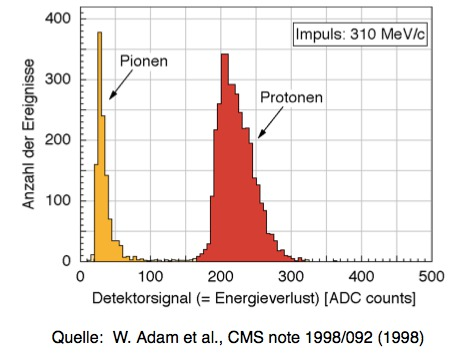
\includegraphics[width=0.5\textwidth]{landau.jpg}
	\caption{Die Energieverteilung des Energieverlustes ist eine Landau-Verteilung.}
	\label{}
\end{figure}

Rarely occuring collisions with small impact parameters lead to tails at high energy transfers. In
this collisions so-called $\delta$-electrons with high energies (keV) are set free. For the mean
loss of energy is higher than the most probable loss of energy, the distribution is asymmetric.
\\
The loss of energy in thin absorbers can be described by a Landau distribution, for thick absorbers,
this merges to a Gaussian distribution.
